% Weaknesses of this chapter include mentions of high-bandwidth system that is not actually ever used. The same can be said for the experimental chapter which discusses its design somewhat.

\documentclass[a4paper]{article}
\usepackage{import}
\subimport{../}{preamble}
\begin{document}

\section{Experimental Measurements of Dynamic Tip Dimers}

% Setup procedure
Dynamic interactions between two tips are spectroscopically studied using an axial scanning approach. Tips are first aligned into the dimer configuration under the supercontinuum laser beam using the capacitive technique described in \ref{sec:tip_alignment}. Alignment takes place with the laser illumination on to prevent spatial changes of the tip apices, caused by thermal expansion, from occurring post-alignment when spectroscopy is performed. The harder tip of the pair is partially positioned in the laser spot and the softer tip is resonantly driven and used as the alignment probe, beginning at distances outside of the laser focus. Ideally sufficient space is left after placement of the stationary tip under the laser spot to accommodate both tip apices equally when brought together. This level of positioning is subjective with scattering intensity used to estimate an acceptable position for the stationary tip within the collection spot. With alignment complete the separation between tips is reduced from around $\sim$\SI{300}{nm} to geometrical contact whilst undergoing measurement.

% Sample preparation
The tips used in experiments, whether commercial or fabricated in-house, are required to have clean metallic surfaces when studying gap plasmon interactions. Layers of insulating chemicals only prevent the gap from narrowing sufficiently or achieving even tunnelling currents. Any layers deposited as either a byproduct of a chemical reaction or carbon deposition in SEM need to be removed. This is done through either plasma cleaning or piranha treatment. To maintain cleanliness some experiments are performed in a nitrogen flow environment.

\begin{figure}[bt]
\centering
\fontsize{10pt}{1em}\selectfont
\def\svgwidth{0.6\textwidth}
\subimport{./figures/}{simple_optics_dimer_layout.tex}
\caption[Experiment configuration for axial tip scanning]{\textbf{Experiment configuration for axial tip scanning.} The laser is centred on the aligned tip dimer for gap spectroscopy. The soft cantilever approaches the stationary, stiff cantilever at a rate $dz$~\si{\nano\metre\per\second}. A bias is applied across the tip junction and the current through the gap is measured. The soft cantilever faces the AFM module for force measurement via cantilever deflection.}
\label{fig:simple_optics_dimer_layout}
\end{figure}

% Procedure
Once two tips are aligned their separation-dependent properties are dynamically probed. The stationary tip acts as the optical probe since it stays fixed in the collection spot through the scan, while the other tip approaches at a rate of 0.1--\SI{1}{\nano\metre\per\second}. Use of a stiffer cantilever ensures that, even when under pressure from the opposite tip, the probe tip remains fixed in its current position under the laser spot. Both optical and electronic properties are simultaneously measured along with the applied force. The geometry of this experiment is shown in \figurename~\ref{fig:simple_optics_dimer_layout}.
% Optics
The approaching tip perturbs the near-field and interacts with the probe tip. Gap-dependent plasmon coupling scatters into the objective collection aperture via outcoupling with plasmonic antenna modes in the probe tip. It is necessary to optimise the scan speed to reduce the time interval between alignment and achieving geometrical contact to minimise any potential drift effects. Strong scattering of the intense supercontinuum source means  \SI{10}{ms} integration times are sufficient for a high quality signal to noise, therefore spectra acquisition does not affect the scan speed. % Not mentioning polarisation sensitivity?

Optical measurements are supplemented by simultaneous electronic and force measurements, enabling correlations in the gap properties to be made.
% Electronics
Electronic properties are probed by driving with a d.c. applied bias and measuring the current through the tip junction to determine its conductivity. A bias of \SI{50}{mV} is almost always used to achieve good signal quality in both the low-bandwidth and high-bandwidth conductance measurements and to prevent spikes in the noise from setting off the high-bandwidth trigger. Larger voltages increase the electrostatic pull between tips, visible in force measurements, and the resulting high current upon contact can damage tips. The current range is limited to above \SI{10}{nA} with a sensitivity of \SI{10}{fA} as lesser ranges require longer settling times, slowing the scan rate. At \SI{50}{mV} the measurable conductance is \orderof{\num{e-7}\G0}. In principle this conductance range is sufficient to accurately survey gaps below $\sim$\SI{0.7}{nm}.
% Force
The applied force is measured using optical detection of the cantilever deflection by the AFM module. At each step in the scan the position of the returning laser beam is averaged for \SI{100}{ms} to determine the mean cantilever deflection, and therefore the mean applied force, over the duration of electronics and optics measurements. % We have a mean but no standard deviations or errors are ever quoted
% Summary
Using this combination of measurements allows for a fuller understanding of nanoscale gap behaviour than by measuring the optical scattering alone.

\subsection{General Properties of a Nano-Tip Dimer Gap}

Before studying the optical properties of nano-gaps it is beneficial to understand the range of physical phenomena that exist on each of the characteristic length scales in scans that traverse from \orderof{\SI{100}{nm}} to \orderof{\SI{0.1}{nm}}. With tips well separated, both the separation and the optical scattering are the only meaningful physical quantities. The optical scattering, if plasmonic in origin, is subject to a separation-dependent capacitive interaction. There is no current and no applied force until the separation reduces to below \orderof{\SI{10}{nm}}. Below this point both the current and the force become instrumental in understanding the optical response. Due to the maturity of AFM, STM and molecular electronics there is already a wealth of information explaining both the electronic and force effects expected on these length scales.

\begin{figure}[bt]
\centering
\includegraphics{figures/tip_scanning_properties}
\caption[Axial force and conductance measurements of a sharp Au tip dimer approaching into contact]{\textbf{Axial force and conductance measurements of a sharp Au tip dimer approaching into contact.} The characteristic AFM snap-in effect is seen as a discontinuous jump before the linear application of force regime. The tip apices snap together, reducing the separation to on the order of \SI{1}{nm}, leading to the onset of quantum tunnelling upon further decreasing the gap separation.}
\label{fig:tip_scan_props}
\end{figure}

\figurename~\ref{fig:tip_scan_props} shows the conductance and axial force measurements from a typical scan once separation has passed below \SI{10}{nm}. The force shows no features until there is a fast negative jump in the applied force, showing that the tip has been pulled in towards the opposing tip (\figurename~\ref{fig:tip_scan_props}a). The lack of a tunnelling current at this point shows that the tip has not yet achieved contact with the opposite tip and must still be separated by more than \SI{1}{nm}. This is the signature of water in gap.

% Snap-in
Since experiments are carried out in ambient conditions the surface of the tips will always be coated in a thin film of water or nanobubbles. Even in a nitrogen environment, water is still present, although the thickness is reduced. When two coated surfaces come into close proximity a water meniscus forms between them, leading to strong capillary forces \cite{gan2009atomic}. Hence, when the separation between the two tips reduces past the point of meniscus formation they are quickly pulled together \cite{holmberg2013}. This is known in AFM literature as the "snap-in" or "snap-into-contact" and occurs on separations $\sim$5--\SI{30}{nm} \cite{holmberg2003, song2014}. In the above scan the snap distance can be inferred from the force as \SI{5}{nm} since this is the amount of approach required to remove the applied force.

To prevent snap-in either a stiffer cantilever must be used (normally in tapping mode) \cite{zhong1993fractured} or the water meniscus has to be removed, which is usually achieved through liquid immersion AFM \cite{hansma1994tapping, putman1994tapping, song2014}, though it can be achieved by using plasma treatment to remove hydrophobic contamination \cite{song2014}. In this case, however, the water layer is advantageous. The presence of the meniscus prevents immediate electrical contact and holds tips apart with $\sim$\SI{1}{nm} gap until further force is applied. This effectively splits a scan into three regimes - one in which the piezo displacement corresponds directly to the separation decrease between tips, one after snap-in where increased displacement neutralises the capillary force and pushes the tip through the water meniscus (soft interaction), and finally one in which force is applied directly to the opposite tip (hard-wall contact).

The existence of the soft interaction regime allows for sub-nm gaps to be studied with some degree of control since only a fraction of the applied cantilever displacement corresponds to a displacement of the apex. Instead, the meniscus is loaded with the applied force leading to the linear reverse deflection observed in AFM force measurements. This can be seen in \figurename~\ref{fig:tip_scan_props} where \SI{15}{nm} of cantilever displacement moves the apex $\sim\SI{0.8}{nm}$ (deduced from electron tunnelling measurements). The remaining \SI{14.2}{nm} loads the gap with an applied force of \SI{8}{nN}, proportional to the tips spring constant.

Use of soft AFM probes (contact mode cantilevers) means a greater spatial resolution in the sub-nm regime since the force required to push through the meniscus is applied more gently for the same size step in cantilever displacement.%
\footnote{Smaller $k$ means larger $x$ required for $F=kx$ to meet the same target value.}
Softer cantilevers are also advantageous during tip alignment as they have larger oscillation amplitudes (lower voltages needed to achieve acceptable signal quality) and lower bandwidth requirements (\SI{13}{kHz} as opposed to 190--\SI{300}{kHz}).
For these reasons, one tip in the dimer is usually a contact mode probe while the other tip, which must remain stationary under an applied force, is a stiffer tapping mode probe. Early experiments exclusively used contact mode probes however spectral changes could not be guaranteed to originate from the gap when under the application of a large force since the whole tip dimer would be displaced from the laser spot.

% Electronics
Despite their usefulness in showing the relative motion of the tip, force measurements are somewhat limited in their information on the absolute separation. An estimate of the absolute separation is made possible by studying charge transfer in the gap.
% Mathematical description of tunnelling
Electron tunnelling is the dominant charge transfer mechanism, occurring prior to geometrical (conductive) contact. The generalised description of this process is given by the Simmon's equation \cite{simmons1963generalized}, which describes the current density $J$ through a tunnelling barrier of width $d$ and arbitrary shape. In many cases it is often simplified using the low-to-zero voltage approximation into \cite{simmons1963generalized},
\begin{equation} J = \frac{3}{2} \frac{(2m\varphi)^{\frac{1}{2}}}{d} \left(\frac{e}{h}\right)^2 V e^{-2({2m\varphi}/{\hbar^2})^{\frac{1}{2}}d},
\end{equation}
where $\varphi$ is the mean barrier height of the assume rectangular barrier. The equation can be considered to be of the form \cite{ tan2014},
\begin{equation} J=J_0e^{-\beta d}, \end{equation}
where $J_0$ is the saturation current density at $d=0$ and,
\begin{equation} \beta = \sqrt{\frac{2m\varphi}{\hbar^2}}, \end{equation}
is the decay rate consisting of the barrier work function $\varphi$. The current due to tunnelling follows an exponential decay with increasing separation therefore the current drops by a factor 10 for every \SI{1}{\angstrom} (\SI{0.1}{nm}) away from geometrical (conductive) contact.

% Charge transfer
Upon reducing the gap to below \SI{1}{nm} electron tunnelling becomes detectable. Though the absolute value of the conductance for a given separation depends on the gap morphology the relative exponential conductance drop from geometrical contact still approximately holds for $d>\SI{2}{\angstrom} $\cite{esteban2014classical}. This makes electron tunnelling a useful method for determining the gap size to within \SI{0.1}{nm}, as is done in STM, though the technique is limited to sub-nm separations. Once the separation is greater than \SI{1}{nm} the conductance drops from $1\G0$ at conductive contact to $10^{-10}\G0$ and the corresponding current becomes difficult to measure without significantly raising the d.c. bias. Use of a large bias of \SI{50}{mV} still means a current on the \orderof{\SI{0.1}{fA}}\footnote{$10^{-16}\si{A}$}, which remains below the noise level achievable in the current setup. Increasing the bias also increasing the electrostatic forces pulling the tips together, therefore decreasing the effective gap resolution in the sub-nm regime.
% effect of water in the gap on tunnelling calibration? effect of finite large surface?

\figurename~\ref{fig:tip_scan_props}b shows a typical conductance trace on approach. Once the separation decreases below \SI{1}{nm} the conductance quickly increases from \num{e-8} to around $10^{-3}\G0$ as the tips transition through the soft interaction regime, at which point the rate of increase slows. {\color{red}This is thought to be caused by displacing the water layer until only a \SI{3}{\angstrom} gap film remains, which may or may not be more solid than the original water film.} A larger force is required to push through this layer and into conductive contact. Once the gap reduces below \SI{2}{\angstrom} there is usually a sharp increase in the current as it transitions into full conductive contact, ranging between $1\G0$ and $200\G0$.

%The use of tunnelling currents as a distance measure also means that the gap size can potentially be stabilised in the sub-nm regime by using a feedback loop, thus operating more like a traditional STM.

Both the force and the conductance provide significant insight into the structure and dynamics of nanoscale gaps. They become especially useful when correlating spectral changes that depend sensitively on gap morphology and dielectric medium. From this information more accurate physical models can be developed to further understand the sub-nm plasmonics regime.

\section{Plasmonic Coupling Between Tips}

\begin{figure}[h]
\centering
\def\svgwidth{0.5\textwidth}
\subimport{./figures/}{tip_dimer_diagram.pdf_tex}
\caption[Diagram of tip dimer characteristics]{\textbf{Diagram of tip dimer characteristics.} The diagram specifically shows the case for a spherical Au tip dimer, showing the antenna plasmon modes which couple together. Plasmonic coupling depends on both the gap size, $d$, and the particle radius, $R$, where the mobile tip particle approaches a stationary spherical tip at a rate $dz$. The illumination and collection geometries are defined by $\vec{k}_{in} = \sin^{-1}(\mathit{NA})$ and $\vec{k}_{scat} < \sin^{-1}(0.8\mathit{NA})$.}
\label{fig:tip_dimer_diagram}
\end{figure}

Plasmonic interactions between tip structures are studied using the dimer approach. Two AFM tips are dynamically brought together to form a single gap structure, mimicking a plasmonic MIM dimer, whilst the optical scattering, conductance and force are simultaneously measured. The resulting experiment geometry during axial tip scans is shown in \figurename~\ref{fig:tip_dimer_diagram}.

% Tips used and the scanning method
The two tip geometries studied using the axial scanning method, arranged in various permutations, are the previously discussed sharp Au tip and spherical Au tip geometries. By comparing the resonances extracted from hyperspectral scans of each individual tip structure to their behaviour in the presence of another resonance the plasmonic properties of tip and tip-gap plasmons can be deduced.

\subsection{Sharp Tip Dimer Interactions}

% Experimental data
\begin{figure}[h]
\centering
\caption[Spectra of a sharp Au tip approaching a stationary sharp Au tip]{\textbf{Spectra of a sharp Au tip approaching a stationary sharp Au tip.} Sharp Au tips are BudgetSensors GB AFM probes. There are no identifiable plasmon resonances initially in the system and no new modes appear with decreasing gap size.}
\label{fig:sharp_tip_scan}
\end{figure}

The first combination of AFM tips studied is a sharp Au tip interacting with another sharp Au tip. Since sharp tips lack the necessary antenna modes, no observable coupling is expected, despite the possibility that a gap mode may exist. Reducing the separation between two sharp Au tips indeed shows no resonances or coupled modes. Some scattering increase is observed, however this correlates with changes in torsional force and therefore corresponds to an increase in light reflected from the tip facet into the objective collection angle. The superimposed spectral scattering increase also bears resemblance to the spectral density of the illumination.

Tunnelling currents are observed to have no effect on scattering from the gap, despite reports suggesting that tunnelling electrons excite SPPs \cite{lambe1976, berndt1991, bharadwaj2011, wang2011, divitt2013, ye2014}. The reason for this is the low bias voltage of \SI{50}{mV}. There is an excitation limit of $h\nu<eV$ to conserve energy \cite{} and hence only low energy SPPs in the IR have a possibility for excitation. Using higher voltages around \SI{2}{V} gives a finite probability that an electron can excite a SPP. The observed intensity then depends on the current through the junction and the collection geometry. In the current geometry only localised gap modes could be observed. Excited SPPs must localise and radiatively decay to be observed in the absence of a $\mathit{NA}>1$ collection geometry.

In this system there is no guarantee that apex localisation should occur and momentum conservation would suggest that SPPs excited via tunnelling electrons would propagate away from the apex.
It is likely that their the voltage is not sufficiently large for the resulting current to excite a large number of scattering plasmons. In typical electrical excitation experiments sensitive CCDs are used with long exposure times around \SI{60}{s} \cite{}. Experiments with the supercontinuum source use \SI{10}{ms} integration times, much too short to see electrical plasmon excitations.

The conclusions drawn from these experiments agree with those of individual sharp Au tip spectroscopy. Sharp Au tips do not show any evidence of supporting antenna plasmon modes and there are no signatures of plasmon coupling emerging from tip dimer scans. However, the gap geometry and external evidence \cite{} points to the existence of gap modes. The lack of their observation therefore supports the argument that antenna modes are required to \emph{efficiently} observe localised plasmons in the far-field. This sets limitations on the experimental geometries necessary to dynamically study plasmons on the sub-nm scale. For this reason the spherical tip geometry, with its visible antenna plasmon, enables the study of gap modes.

\subsection{Spherical Tip Dimer Interactions}

By using spherical Au tips the tip-tip system mimics the prototypical spherical AuNP dimer. It is through this  arrangement that a dynamically controllable plasmonic dimer is {\color{red}recreated/created/formed} from which plasmon coupling can be studied. The presence of antenna modes, discussed in \ref{ch:tip_plasmonics}, enables the detection and study of gap modes as the gap size transitions from the non-interacting regime at $\sim\SI{300}{nm}$ down to the charge transfer regime at or before geometrical/conductive contact. By utilising such a controllable plasmonic system nanoscale plasmon coupling can be better understood on a fundamental level and unravel the remaining questions regarding plasmonics in the sub-nm gap regime.

\subsubsection{Spherical Tip Interactions with a Spherical Tip}

\begin{figure}
\centering
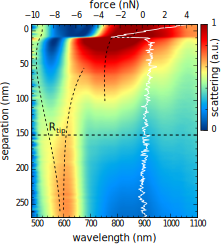
\includegraphics{figures/classical_tip_dimer_1}~
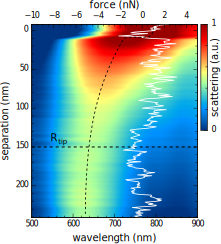
\includegraphics{figures/classical_tip_dimer_2}
\caption[Spectra of a spherical Au tip approaching a stationary spherical Au tip]{\textbf{Spectra of a spherical Au tip approaching a stationary spherical Au tip.} Spherical Au tips are Au-coated NanoTools B150 AFM probes. With similar initial plasmon resonances bonding hybridised modes form, which redshift with increased coupling/decreasing gap size.}
\label{fig:spherical_tip_dimer_scan}
\end{figure}

The first configuration of spherical tips studied is that of a spherical Au tip approaching another spherical Au tip. In this instance the 600--\SI{650}{nm} antenna plasmons of the individual tips interact and form far-field observable hybridised gap modes. Coupling between spherical tips appears very similar to that of a large nanoparticle dimer. As the gap width decreases the individual plasmon modes mostly couple into bonding hybridised modes that redshift monotonically and scatter increasingly (\figurename~\ref{fig:spherical_tip_dimer_scan}). The increased scattering is due to both an increasing coupling and an increased amount of scattering metal entering the {\color{red}confocal sampling volume of the objective}. Once the gap has decreased sufficiently ($d \ll d_{sph}$) the confocal collection argument is negligible as the sampling volume becomes saturated, hence all further changes occur due to plasmon coupling in the gap.

For large distances the rate of redshift is dominated by the increase in capacitive coupling as the separation decreases. In each scan a large abrupt redshift of the coupled mode correlates with the snap-in effect measured by the AFM. Snap-in confirms the presence of water layers in the gap meaning a transition is expected from an air gap medium to a higher refractive gap medium containing water and any organic contaminants pulled into the gap by the water meniscus. The large redshift on snap-in is due in part to two effects: the decrease in separation as the tip is pulled in by {\color{red}capillary/meniscus} forces and the increase in refractive index as the gap constitution becomes all water.

The intensity of the lowest order mode increases with coupling until the gap separation is below \SI{1}{nm} at which point it begins the decrease. This effect is attributed to the mode being confined to such a degree that it becomes increasingly less radiative as this effect occurs before the onset of any significant quantum effects. From theory it has been seen that the field enhancement in the gap continues to increase despite the intensity decrease, confirming that the gap mode still exists but with lower radiative emission \cite{esteban2012}. To some extent this can be considered to be because the charge localises so strongly at the gap, increasing the field enhancement, that the antenna mode is reduced by the skewing.

\begin{figure}[h]
\centering
\includegraphics{figures/classical_mode_fits}
\caption[LSP resonance wavelengths and amplitudes over multiple scans of spherical tip dimers]{\textbf{LSP resonance wavelengths and amplitudes over multiple scans of spherical tip dimers.} The antisymmetric nature of the system mimics a heterodimer leading to the observation of both bonding (red) and anti-bonding (blue) hybridised modes.}
\label{fig:heterodimer_measurements}
\end{figure}

Slightly different classical coupling physics is observed if the dimer symmetry is broken. In some cases where the resonances of the particles differ by $\sim\SI{50}{nm}$ the scattering/plasmon coupling is described by the heterodimer model rather than the more common homodimer. In this situation anti-bonding modes are no longer dark since dipoles do not exactly cancel. Depending on which particle is probed, the lower or higher energy initial resonance, either a redshifting bonding mode or a blueshifting then redshifting anti-bonding mode will be observed (see \figurename~\ref{fig:plasmon_hybridisation}). These two types of hybridised modes are seen across many different scans (\figurename~\ref{fig:heterodimer_measurements}).

This effect has been documented previously \cite{nordlander2004} but never directly observed dynamically. The anti-bonding configuration is typically non-physical in most plasmonic systems since both particles are driven with the same phase of light. However, with larger particles, such as the $R=\SI{150}{nm}$ spherical tips, and with higher order resonances the phase symmetry is broken allowing an anti-bonding configuration to be excited. {\color{red}The hybridised mode therefore blueshifts with increasing coupling until the coupling increases sufficiently to force the mode into phase, at which point the mode begins to redshift.}

\subsubsection{Spherical Tip Interactions with a Planar Surface}

\begin{figure}[h]
\centering
\caption[]{Spectra of a spherical Au tip approaching a Au planar surface (AFM cantilever). No coupling phenomena are observed.}
\label{fig:spherical_tip_cantilever_scan}
\end{figure}

By reversing the stationary AFM probe in its mount its cantilever is exposed to the opposing tip. The end of the cantilever is placed in the sampling volume so as the maximise the amount of light penetrating the focal spot around the cantilever width. Scattering from the Au-coated cantilever is minimal and insignificant compared with that of the spherical tip apex. The spherical tip is approached towards the cantilever and measurements taken (\figurename~\ref{fig:spherical_tip_cantilever_scan}).

Force measurements confirm contact between the tip and the cantilever.

\subsubsection{Spherical Tip Interactions with a Sharp Tip}

The interaction between the same AuNP tip and a sharp Au tip is investigated. The results are shown in \figurename~\ref{fig:spherical_sharp_tip_scan}.

\begin{figure}[h]
\centering
\includegraphics{figures/sharp-AuNP_tip_dimer}
\caption[Spectra of a spherical Au tip approaching a stationary sharp Au tip]{\textbf{Spectra of a spherical Au tip approaching a stationary sharp Au tip.} No coupling phenomena are observed due to the mismatch between localised surface plasmon modes.}
\label{fig:spherical_sharp_tip_scan}
\end{figure}

Despite the sharp tip perturbing the field around the spherical tip acting as the optical antenna, no changes are observed in the spherical tip plasmon, suggesting that there is no interaction between sharp tips and spherical tip plasmons.
{\color{red}The observation of no coupling somewhat makes sense in that a mode will only interact with a similar mode in the opposing nanostructure \cite{nordlander2004}.} A nanoparticle can therefore couple with another nanoparticle or its image in a surface, since only a real particle or image can sustain a similar mode. A sharp tip does not have the means of supporting a LSP mode similar to that of the spherical tip in the sense that it has no polar antenna modes nor the planar surface area to form image an charge distribution, hence the spherical tip mode does not couple or redshift.

%\subsubsection{Spherical Tip TERS}

\section{Quantum Effects in Sub-nm Gaps between Spherical-Tipped AFM Probes}

Should the surface of the two approaching spherical surfaces be clean enough that the formation of a sub-nm gap becomes possible, the influence of quantum effects on plasmonic coupling becomes readily observable. By monitoring the electrical conductivity simultaneously with the optical scattering the effect of a tunnelling current on plasmon coupling can be directly inferred.

For a metal-air-metal interface, or more likely for gaps in ambient conditions, a metal-water-metal interface, the onset of electron tunnelling begins at increased distances of $d \sim \SI{0.9}{nm}$. At d.c. frequencies it is assumed that tunnelling conductances decrease by an order of magnitude per angstrom moved away from the point of metal-metal contact. This is the STM model of tunnelling. The absolute value of conductance on contact in such large junctions is debatable since the integrated tunnelling becomes comparable to the conductance of a single atom contact. Nevertheless the d.c. tunnelling conductance gives a good indication of the gap size as well as an estimation of what the a.c. optical conductivity of the plasmonic gap may be.

%\begin{figure}[h]
%\centering
%\begin{subfigure}[t]{0.49\textwidth}
%	\includegraphics[width=\textwidth]{figures/old_ball_tip_dimer_scan}
%	\caption{Spherical Au tips (Au-coated NanoTools B150 ball tips).} \label{fig:old_ball_tip_scan}
%\end{subfigure}
%\begin{subfigure}[t]{0.49\textwidth}
%	\includegraphics[width=\textwidth]{figures/echem_tip_dimer_scan}
%	\caption{Electrochemically fabricated AuNP-on-Pt tips (asymmetric morphology, hence more modes and visibility of dark modes).} \label{fig:old_ball_tip_scan_analysis}
%\end{subfigure}
%\caption{Correlated measurements of spectra, tunnelling conductance and force during reduction of tip separation (gap size) in the sub-nm regime.}
%\end{figure}

% Observation of different phenomena
\begin{figure}[h]
\centering
\begin{subfigure}[t]{0.4\textwidth}
	\flushright
	\includegraphics{figures/orig_spherical_tip_dimer_tunnelling_focus}
	%\caption{}
	\label{fig:scan1}
\end{subfigure}
~
\begin{subfigure}[t]{0.4\textwidth}
	\flushleft
	\includegraphics{figures/echem_tip_dimer_tunnelling_focus}
	%\caption{}
	\label{fig:scan2}
\end{subfigure}
\\
\begin{subfigure}[b]{0.4\textwidth}
	\flushright
	\includegraphics{figures/spherical_tip_dimer_1_tunnelling_focus}
	%\caption{}
	\label{fig:scan3}
\end{subfigure}
~
\begin{subfigure}[b]{0.4\textwidth}
	\flushleft
	\includegraphics{figures/spherical_tip_dimer_2_tunnelling_focus}
	%\caption{}
	\label{fig:scan4}
\end{subfigure}
\caption[Scans of multiple spherical tip dimers pushing towards geometrical contact and showing varying phenomena]{\textbf{Scans of multiple spherical tip dimers pushing towards geometrical contact and showing varying phenomena.} Scans show the supercontinuum dark-field scattering spectra as a function of the applied force on the gap with the simultaneously measured conductance superimposed over the axis. The circles highlight the position an evenly distributed selection of the peak position. The size of the circle indicates the amplitude of the mode in the fitted model. Scans a,c and d use Au-coated NanoTools B150 spherical AFM probes to form a dimer while scan b uses electrochemically-fabricated AuNP-on-Pt AFM tips.}
\label{fig:spherical_tip_scans}
\end{figure}

\figurename~\ref{fig:spherical_tip_scans} shows a selection of spherical tip scans showing simultaneous quantum tunnelling and supercontinuum dark-field scattering measurements, in which each scan shows varying phenomena when in the tunnelling regime. Each of the scans shows similar behaviour in the classical, capacitive coupling regime, therefore changes in the plasmonics are thought to derive from sub-nm scale physics.
% The explanation of different phenomena
% Screening and blueshifting
Both \figurename~\ref{fig:scan1} and \figurename~\ref{fig:scan3} show the screening and blueshifting of the higher order mode. While this behaviour is expected as the tunnelling increases the scans are different in that the screening occurs once $G>10^{-3}G_0$ in \figurename~\ref{fig:scan1} whereas screening only occurs once $G>G_0$ in \figurename~\ref{fig:scan3}. Despite quantised conductance steps being observed in \figurename~\ref{fig:scan3} there is no obvious step-wise behaviour in the optics.

%\begin{wrapfigure}{O}{0.5\textwidth}
\begin{figure}[bt]
\centering
\includegraphics{figures/qcm_tip_theory_zoom}
\caption[Select view of calculated QCM spherical tip dimer spectra as a function of separation \cite{savage2012}]{\textbf{Select view of calculated QCM spherical tip dimer spectra as a function of separation \cite{savage2012}.} Simulated spectra show that the higher order mode disappears and a CTP mode rises prior to geometrical contact at $d_{QR}=\SI{0.3}{nm}$. This occurs since coherent electron tunnelling transfers sufficient charge to excite a CTP mode and screen out the capacitively coupled (bonding) modes.}
\label{fig:qcm_tip_theory}
\end{figure}
%\end{wrapfigure}

% Power transfer
Figures \ref{fig:scan2} and \ref{fig:scan4} show a different set of phenomena. No clear screening of a single mode is observed in these scans through the tunnelling regime. Instead the higher order mode simply decreases in intensity as a second (CTP) mode rises (\figurename~\ref{fig:scan2}). The CTP mode is excited at a higher energy than the coupled mode. This is similar to the scan in \figurename~\ref{fig:scan4} except that the higher order coupled mode blueshifts slightly and the CTP emerges at a lower energy.

% The explanation of different phenomena
The power transfer effect shown in \figurename~\ref{fig:scan2} bears similarity with the formation of the higher order CTP mode in the QCM calculations (\figurename~\ref{fig:qcm_tip_theory}). Fitting the spectra in \figurename~\ref{fig:scan2} shows a linear rate of change in the amplitude of both the coupled and CTP modes with the area under both curves conserved. This indicates that electrons are directly transferring from the coupled mode to the CTP mode.

\FloatBarrier
\begin{figure}
\centering
%\fcapside[\FBwidth]
{\includegraphics{figures/tunnelling_plasmonics_diagram}}
{\caption[Diagram of possible plasmonic gap configurations in the tunnelling regime]{\textbf{Diagram of possible plasmonic gap configurations in the tunnelling regime.} An ideal symmetric dimer surface (a) will have perfect overlap between the plasmon mode and the point tunnelling leading to field screening. Roughened surfaces have a statistically high chance of conforming to the symmetric configuration (b) or the roughness may lead to localisation of the point of tunnelling to outside the plasmonic hotspot (c).}
\label{fig:tunnelling_plasmonics_diagram}}
\end{figure}

% Idealistic smooth surfaces
The hypothesis linking the scans together is that the spatial location of the point or points of conduction in relation to the gap plasmon field is of significant importance. For two ideal (smooth) surfaces coming together the symmetry of the system means that both the gap plasmon field and the shortest conduction path between surfaces are coincident (\figurename~\ref{fig:tunnelling_plasmonics_diagram}a). In this case the optical response is likely to reflect that of QCM spectra \cite{savage2012} (\figurename~\ref{fig:qcm_tip_theory}) with both the emergence of a tunnelling CTP and the gap plasmon modes being screening, and therefore blueshifting, with the increase in tunnelling current.
% Realistic rough but aligned surface
For a more realistic surface that includes atomic to nanoscale roughness there is statistically a good chance that the plasmon field and the shortest conduction path {\color{red}overlap/align} (\figurename~\ref{fig:tunnelling_plasmonics_diagram}b). The physics in this case, to a certain extent, retains the characteristics of the QCM model. It is possible that roughness further localises the gap plasmon in places leading to an inhomogeneous plasmon field but these locations would also likely incur a larger tunnelling current.

% Power transfer without blueshift
Discrepancies between the QCM model and the experimental data occur if the point of conduction does not overlap well with the plasmon field, in which case the field is not screened (\figurename~\ref{fig:tunnelling_plasmonics_diagram}c). The argument that the plasmon field localises most strongly around the region of smallest gap only extends so far as the plasmon will still be more distributed than the conduction path.%
\footnote{$w_{gLSP}=\sqrt{Rd}$ for a gap plasmon and $w_{c}\propto R$ for conduction, hence the gap plasmon is more laterally distributed.}
There is a finite plasmonic density of states, however, and so an electron may either accumulate at the metal/gap interface or tunnel across the gap as part of the tunnelling CTP. Under these conditions it is expected that the number of electrons in the CTP mode increases with the d.c. tunnelling current as the gap barrier width decreases. The number of electrons remaining in the coupled mode must then decrease at the same rate to conserve the number of electrons in the overall structure. Under these circumstances only the intensity of the coupled mode is required to decrease. There is no mechanism which necessitates the screening and blueshifting of the coupled modes.
% Link back to the blueshift case
Furthermore, for the case where the tunnelling results in plasmon screening, there is no reason that the mode amplitude should be conserved during the transition between coupled and CTP modes. Even though the charge must be conserved the contribution of the reduction in coupling to the mode amplitude is entangled with the transfer of charge between plasmon states.

\begin{figure}[h]
\includegraphics{figures/echem_tip_dimer_tunnelling_focus_2}
\caption[]{}
\label{fig:gap_morphology_modification}
\end{figure}

Evidence of the sensitive dependence on gap morphology can be seen in \figurename~\ref{fig:gap_morphology_modification} where the tip is retracted slightly after electrical contact and then approached again. The charge transfer is observed at a lower conductance due to the first electrical contact modifying the gap morphology.

% Summary
To summarise, all cases of charge transfer result in the formation of CTP modes, combined with the decrease of coupled mode intensity to conserve charge. However, only gap configurations in which the current passes through the region in which the gap plasmon should be localised have the effect of screening the coupled modes and reducing the coupling strength. The plasmon field is expelled outwards from the point of contact, forming modes resembling the crevice modes of contacted particles, despite the lack of geometrical contact.

\emph{How do results compare with theory when using high powers like a Fianium? Compare to \cite{marinica2012}.}

\end{document}